%----------------------------------------
% Write your notes here
%----------------------------------------

\section{Introduction}
This is where your text goes.
If you're new to \LaTeX, check out Overleaf\footnote{\url{http://overleaf.com}}, an online \LaTeX~environment where you can edit and render your documents.
They also have a very useful \href{http://www.overleaf.com/help/18-how-do-i-use-overleaf}{getting started guide}.

Figure \ref{fig:example_figure} is an example of how to include an image.

\begin{figure}[ht]
  \begin{center}
    
\includegraphics[width=0.5\textwidth]{figures/example_figure.png}
    \caption{
      This is how to include a figure.
      As long as you use pdflatex most file types (e.g., jpg, png, pdf) should work.}
    \label{fig:example_figure}
  \end{center}
\end{figure}

And here's some math:
\begin{equation}
  \int_{-\infty}^{+\infty} e^{-x^2} dx = \sqrt{\pi}
\end{equation}

You can also make numbered lists:
\begin{enumerate}
  \item Thing 1
  \item Thing 2
  \item etc.
\end{enumerate}

Or bulleted lists
\begin{itemize}
  \item Thing 1
  \item Thing 2
  \item etc.
\end{itemize}

It shouldn't get much more complicated than that.


The two main criteria for evaluating credibility of a research is the reproducibility and replicability of the results. Reproducibility is the ability to independently verify the exact results using the same data and the same analysis. 
This is improving with better software engineering practices among researchers like:
\begin{enumerate}
  \item Literate programming (Jupyter, Rmarkdown)
  \item Automated build scripts (Make_les)
  \item Containers (Docker, Code Ocean)
\end{enumerate}




The well renowned journals like NIPS started to encourage researchers by attaching acknowledgement badges on their published papers as shown in the below picture. 

Figure \ref{fig:badges} is an example of how to include an image.

\begin{figure}[ht]
  \begin{center}
    
\includegraphics[width=0.5\textwidth]{figures/badges.png}
    \caption{
    NIPS Badges
      }
    \label{fig:badges}
  \end{center}
\end{figure}
















 \begin{figure}[ht]
  \begin{center}
    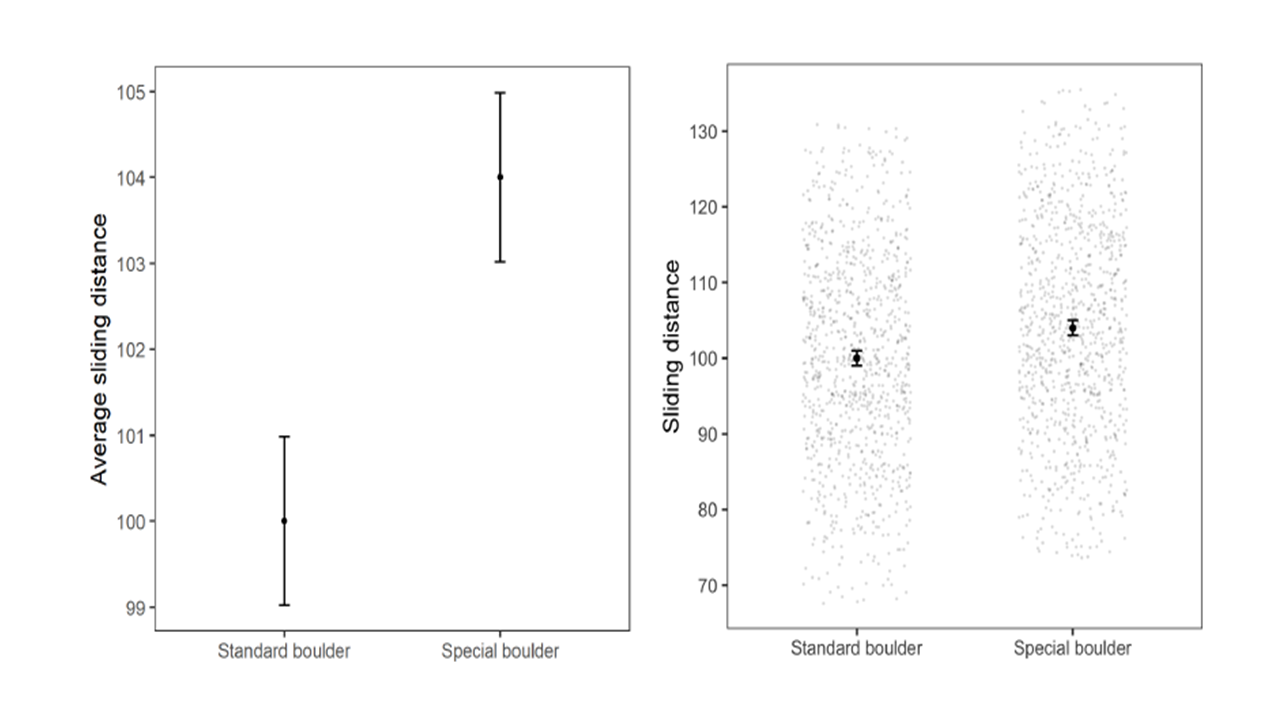
\includegraphics[width=0.5\textwidth]{figures/quiz3.png}
    \caption{
    Left: Bad visualization Right: Correct visualization
      }
    \label{fig:badges}
  \end{center}
\end{figure}
 
 